\chapter{Introduction to DUNE}
\label{ch:exec-overall}

\fixme{For Ed and Stefan}

%%%%%%%%%%%%%%%%%%%%%%%%%%%%%%%%%%%%%%%%%%%%%%%%%%%%%%%%%%%
\section{(Needs section heading)}
\label{sec:exec-overall-1}

The Deep Underground Neutrino Experiment (DUNE) will be a world-class neutrino observatory and nucleon decay detector designed to answer fundamental questions about the nature of elementary particles and their role in the universe. The international DUNE experiment, hosted by the U.S. Department of Energy's \fnal{}, will consist of a far detector to be located about \SI{1.5}{km} underground at the Sanford Underground Research Facility (\surf) in South Dakota, USA, at a distance of  \SI{1300}{\km} from \fnal{}, and a near detector to be located at \fnal in Illinois. The far detector will be a very large, modular liquid argon time-projection chamber (\lartpc) with a \fdfiducialmass (\SI{40}{\giga\gram}) fiducial mass. This \lar technology will make it possible to reconstruct neutrino interactions with image-like precision and unprecedented resolution. 

The DUNE detectors will be exposed to the world's most intense neutrino beam originating at \fnal{}. A high-precision near detector, located \SI{575}{m} from the neutrino source on the \fnal site, will be used to characterize the intensity and energy spectrum of this wide-band beam. The Long-Baseline Neutrino Facility (LBNF), also hosted by \fnal, provides the infrastructure for this complex system of detectors at the Illinois and South Dakota sites. LBNF is responsible for the neutrino beam, the deep-underground site, and the infrastructure for the DUNE detectors. 

\begin{dunefigure}[DUNE collaboration global map]{fig:map2}{The international DUNE
collaboration. Countries with DUNE membership are shown in orange.}
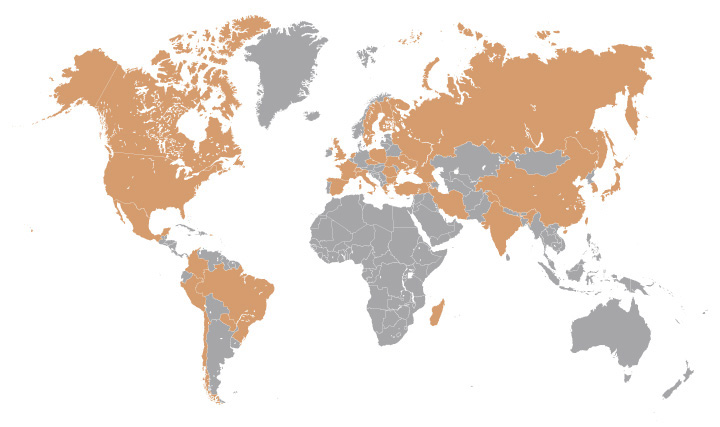
\includegraphics[width=0.9\textwidth]{global-retouched.jpg}  
\end{dunefigure}

The DUNE collaboration is a truly global organization including more than \num{1000} scientists and engineers from \num{31} countries (Figure~\ref{fig:map2}). It represents the culmination of several worldwide efforts that developed independent paths toward a next-generation long-baseline (LBL) neutrino experiment over the last decade. It was formed in April 2015, combining the strengths of the LBNE project in the USA and the LBNO project in Europe, adding many new international partners in the process. DUNE thus represents the convergence of a substantial fraction of the worldwide neutrino-physics community around the opportunity provided by the large investment planned by the U.S. Department of Energy (DOE) and \fnal to support a significant expansion of the underground infrastructure at \surf in South Dakota, and to create a megawatt neutrino-beam facility at \fnal by 2026. The Proton Improvement Plan-II (PIP-II) upgrade at \fnal~\cite{pip2-2013} will enable the accelerator to drive the new neutrino beamline with a \SI{80}{\GeV} primary proton beam at a beam power %from \SI{1.07}{\MW} 
up to \pipiibeampower{}. A further planned upgrade 
of the accelerator complex will enable it to provide up to \SI{2.4}{\MW} of beam power by 2030. 

The LBNF/DUNE project (the \textit{project}) strategy presented in this TDR has been developed to meet the requirements set out in the report of the Particle Physics Project Prioritization Panel (P5 in 2014). It also takes into account the recommendations of the European Strategy for Particle  Physics (ESPP) adopted by the CERN Council in 2013, which classified the \dword{lbl} neutrino program as one of the four scientific objectives that require international infrastructure.
%which recommends development of
%a program to pave the way for a substantial European role in future long-%baseline experiments.

The P5 report~\cite{p5report} set the goal of reaching a sensitivity to \dword{cpv} of better than three standard deviations (\num{3}$\sigma$) over more than $75\%$ 
of the range of possible values of the unknown \dshort{cp}-violating phase \deltacp.
Based partly on this goal, they stated that ``the 
minimum requirements to proceed are the identified capability to reach an exposure 
of \num{120}~\ktMWyr{} by the 2035 time frame, the far detector situated underground 
with cavern space for expansion to at least \fdfiducialmass \lar fiducial volume, and \SI{1.2}{MW} 
beam power upgradeable to multi-megawatt power.
The experiment should have the demonstrated 
capability to search for \dwords{snb} and for proton decay, providing a significant 
improvement in discovery sensitivity over current searches for the proton lifetime.'' The strategy and design presented in this TDR meet these requirements.
%Based on the resource-loaded schedules for the reference designs of the facility %(\vollbnf)
%and the detectors, %(\voldune), 
%the strategy presented here meets these criteria. 


This multi-volume document is the Technical Design Report (TDR) for the DUNE Far Detector. It is intended to provide a clear statement of the physics goals of the DUNE experiment, and to describe the detector designs that we believe will achieve these goals. The TDR includes dedicated volumes on the DUNE physics program, the DUNE far detectors, and the DUNE Technical Coordination organization. This executive summary volume includes less technical overviews of the other volumes. There are also dedicated chapters on the near detector and computing, which will be the subject of future TDRs.

\section{Primary Science Goals (Stefan)}


The DUNE experiment will combine the world's most intense neutrino beam, a deep underground site, and massive LAr detectors to enable a broad science program addressing some of the most fundamental questions in particle physics. 

%The Deep Underground Neutrino Experiment (DUNE) will address the key questions in neutrino physics, will provide a next-generation observatory for astrophysical neutrinos, and will extend the search for baryon number violating processes in particle physics.

%Searches for CP violation in neutrino oscillations may give insight into the origin of the matter-antimatter asymmetry, one of the fundamental questions in particle physics and cosmology. Detection of neutrinos from a nearby supernova could provide a wealth of information about neutrinos and the dynamics of supernovae. Observation of proton decay would dramatically change our understanding of particle physics

The primary science goals of DUNE, described in detail in Chapter~\ref{ch:exec-summ-physics}, are to: 
\begin{itemize}

\item Carry out a comprehensive program of neutrino oscillation measurements using \numu and \anumu beams from \fnal. This program includes measurements of the  \dword{cp} phase, determination of the neutrino mass ordering (the sign of \dm{31}$ \equiv m_3^2-m_1^2$), measurement of the mixing angle $\theta_{23}$ and the determination of the octant in which this angle lies,
and sensitive tests of the three-neutrino paradigm. Paramount among these is the search for \dword{cpv} in neutrino oscillations, which may give insight into the origin of the matter-antimatter asymmetry, one of the fundamental questions in particle physics and cosmology. 

\item Search for proton decay in several important decay modes. The observation of proton decay would represent a ground-breaking discovery in physics, providing a key requirement for grand unification of the forces. 

    \item Detect and measure the $\nu_\text{e}$ flux from a core-collapse supernova within our galaxy, should one occur during the lifetime of the DUNE experiment. Such a measurement would provide a wealth of unique information about the early stages of core-collapse, and could even signal the birth of a black hole.
    
\end{itemize}

The intense neutrino beam from LBNF, the massive DUNE \lartpc far detector, and the high-resolution
DUNE near detector will also provide a rich ancillary science program, beyond the primary goals of the experiment. The ancillary science program includes
\begin{itemize}
     \item other accelerator-based neutrino flavor transition measurements with sensitivity to beyond the standard model (BSM) physics, such as non-standard interactions (NSIs), Lorentz violation,  \dword{cpt} violation, sterile neutrinos, large extra dimensions, heavy neutral leptons;
 and measurements of tau neutrino appearance;
     \item measurements of neutrino oscillation phenomena using atmospheric neutrinos;
     \item a rich neutrino interaction physics program utilizing the DUNE near detector, including a wide-range of measurements of neutrino cross sections, studies of nuclear effects; %, including neutrino final-state interactions, measurements of the structure of nucleons, and  measurement of $\sin^2\theta_\text{W}$;
     \item  searches for dark matter.
\end{itemize} 
Further advancements in the \lartpc %far detector 
technology during the course of the DUNE far detector construction may open up the opportunity
to observe very low-energy phenomena such as solar neutrinos or even the diffuse supernova neutrino flux.


%%%%%%%%%%%%%%%%%%%%%%%%%%%%%%%%%%%%%%%%%%%%%%%%%%%%%%%%%%%%%%%
\section{The LBNF Facility (Elaine?)} 

The Long-Baseline Neutrino
Facility (LBNF), hosted by Fermilab, is separate from the DUNE collaboration and is intended to enable the construction and operation of the DUNE detectors in South Dakota and Illinois.
The DUNE collaboration will construct a deep-underground neutrino observatory in South Dakota based on four independent \nominalmodsize \lartpc{}s. % at \surf. %the Sanford Underground Research Facility (\surf) in South Dakota.
LBNF will provide facilities in Illinois and South Dakota to enable the scientific program of DUNE.
These facilities are geographically separated into the near site facilities, those to be constructed
at \fnal, and the far site facilities, located at \surf. Figure~\ref{fig:lbnf} shows
a schematic of the facilities at the two sites, and Figure~\ref{fig:caverns} shows the cavern layout. 

\begin{dunefigure}[ 	
LBNF/DUNE project: beam from Illinois to South Dakota]{fig:lbnf}{ 	
LBNF/DUNE project: beam from Illinois to South Dakota.}
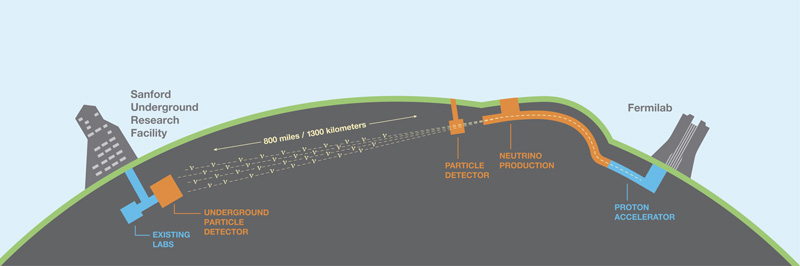
\includegraphics[width=0.9\textwidth]{lbnf_dune_graphic_miles_km-15-0031-01.jpg}
%\label{fig:mhexec}
\end{dunefigure}

Specifically, the Long-Baseline Neutrino Facility (LBNF) provides
\begin{itemize}

\item  the  technical and conventional facilities for a powerful \MWadj{1.2} neutrino beam utilizing the PIP-II upgrade of the \fnal accelerator 
complex, to become operational by \beamturnon  
at the latest, and to be upgradable to \SI{2.4}{\MW} with the proposed 
PIP-III upgrade;

\item  the civil construction, or \dword{cf}, for the near detector systems at \fnal; (see Figure~\ref{fig:beamline}); 

\item the excavation of three underground caverns at \surf, planned to be completed by xxxx. The north and south caverns will each house two cryostats with a
a minimum \nominalmodsize fiducial mass \lartpc, while the central utility cavern will house cryogenics and daq facilities for all four detector modules;



\item surface, shaft, and underground infrastructure to support 
the outfitting of the caverns with four free-standing, steel-supported cryostats 
and the required cryogenics systems. The first cryostat will be available for filling, after installation of the detector components, by
xxxx, enabling a rapid deployment of the first two \nominalmodsize far detector modules. 
The intention is to install the third and fourth cryostats as rapidly as funding will 
allow.

\end{itemize}

\begin{dunefigure}[ 	
Underground caverns for DUNE in South Dakota]{fig:caverns}{Underground caverns for DUNE far detectors and cryogenic systems at \surf{}, in South Dakota.}
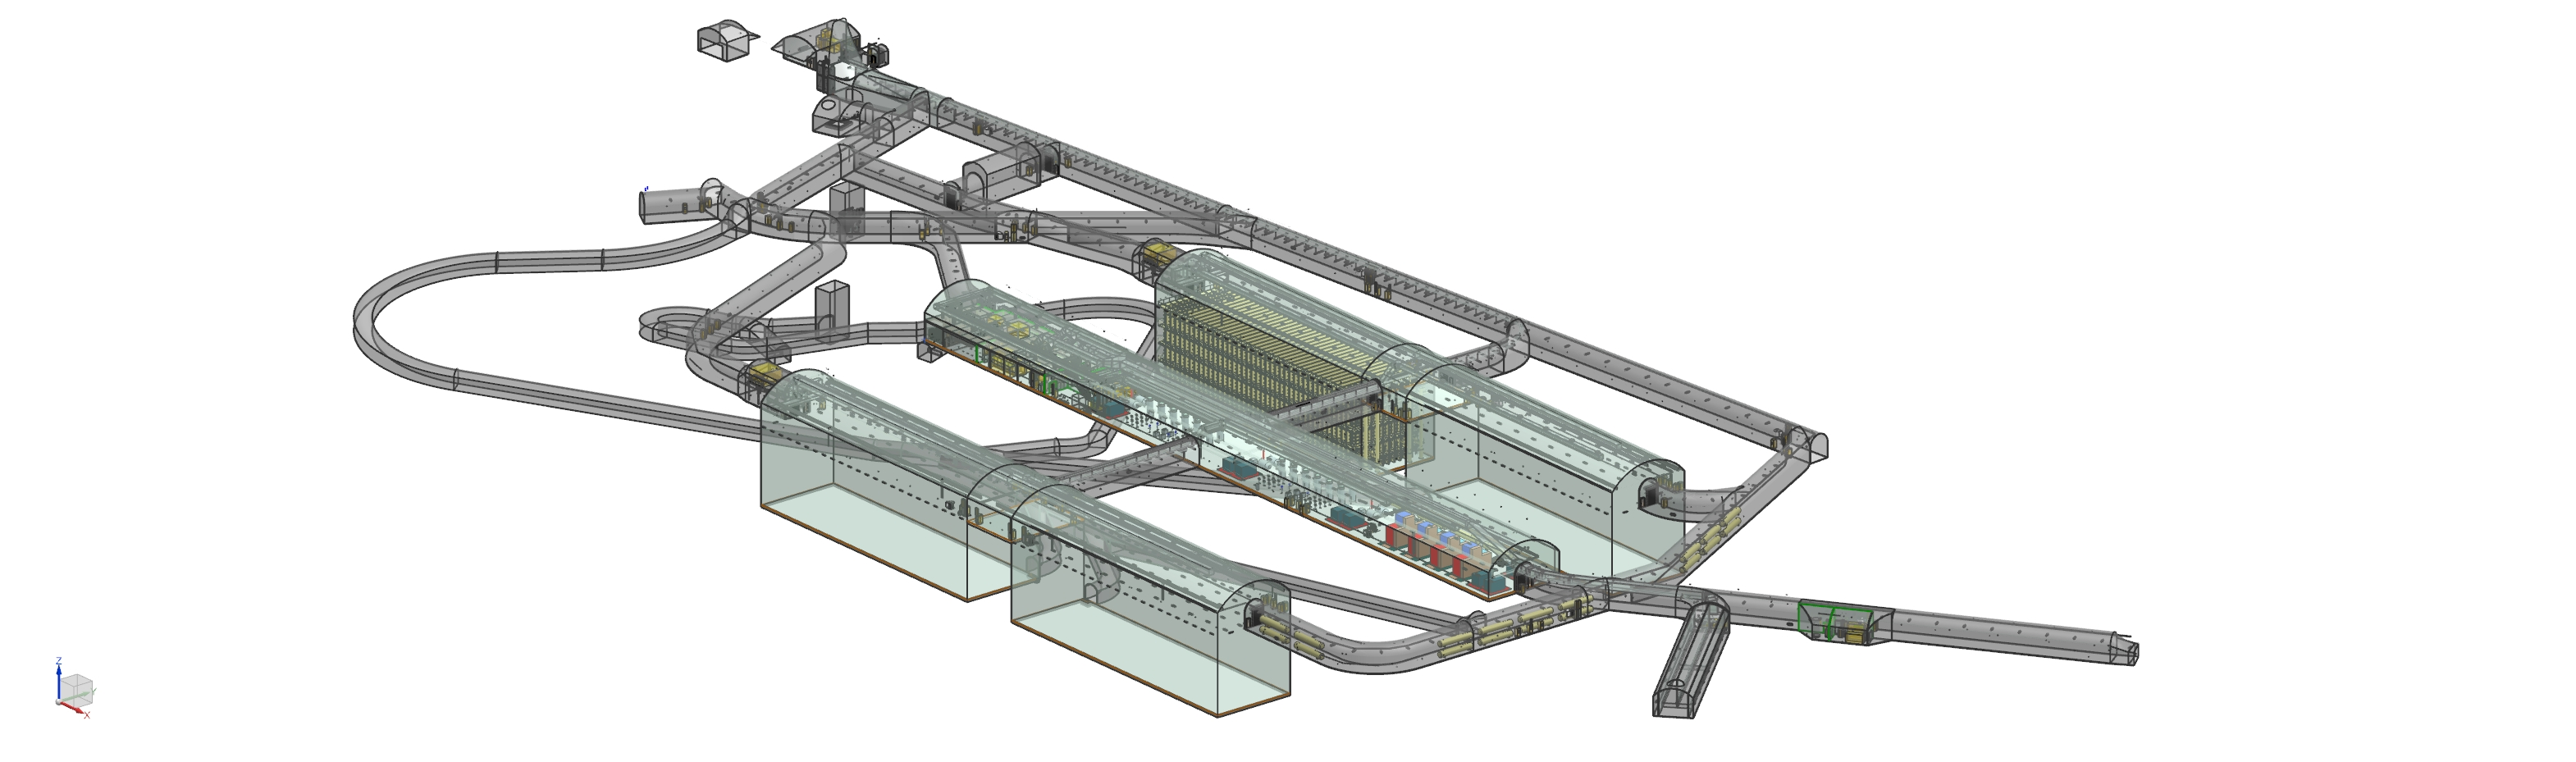
\includegraphics[width=0.95\textwidth]{far-detector-configuration-hi-res.jpeg}
\end{dunefigure}

\begin{dunefigure}[Neutrino beamline and DUNE near detector hall in Illinois
]{fig:beamline}{Neutrino beamline and DUNE near detector hall at Fermilab, in Illinois}
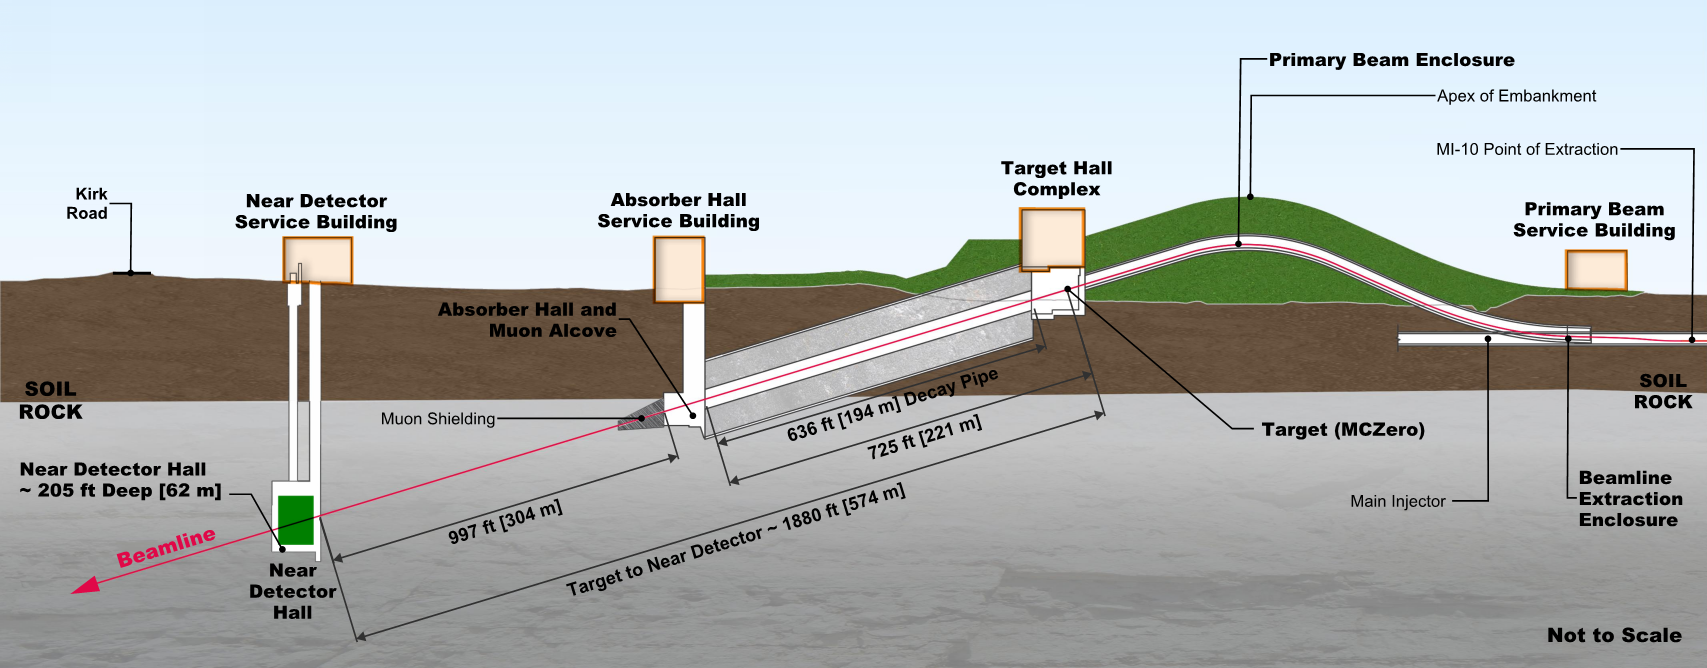
\includegraphics[width=0.95\textwidth]{beamline-sideview.jpg}
\end{dunefigure}


The success of the DUNE project depends on the successful realization of the LBNF facilities.
This \dword{tp} focuses on the DUNE physics program that is enabled by
the first three \dword{fd} modules, which are expected to be based on the \dword{sp} and \dword{dp} \lar technologies. 

\section{The DUNE Experiment} (Ed)

The DUNE experiment includes a precision near detector at the edge of the \fnal site, in Batavia, Illinois, and a very large, modular far detector about \SI{1.5}{km} underground at \surf in Lead, South Dakota, \SI{1300}{km} (\SI{800}{miles}) from \fnal. The DUNE far detector is the focus of this \dword{tdr}. 

% ecb: Do ProtoDUNEs show up here or in a separate section? Somewhere, we need to state what specific performance measures we are counting on having from ProtoDUNE before the TDR.

\subsection{Far Detector (SP/DP?)}

The DUNE \dword{fd} will consist of four similar \lartpc{}s, each with fiducial mass of at least \nominalmodsize, installed about \SI{1.5}{km} underground. Each detector will be installed in a cryostat with internal dimensions
\cryostatwdth (W) $\times$ \cryostatht (H) $\times$ \cryostatlen (L), and will contain a total \lar{} mass of about \larmass{}.
The \lartpc technology provides
excellent tracking and calorimetry performance, making it an ideal
choice for the DUNE far detectors. The four identically sized cryostats give flexibility for staging and evolution of the \lartpc technology.

DUNE is planning for and prototyping two \lartpc technologies:
\begin{itemize}
\item Single-phase (SP): This technology was pioneered by the ICARUS project, and after several decades of worldwide R\&D, is now a mature technology. It is the technology used for \fnal{}'s currently operating \microboone, and the planned SBND. In the \single technology, ionization charges are drifted horizontally in \lar and read out on wires in the liquid. The maximum drift length in the DUNE \dword{spmod} is \spmaxdrift and the nominal drift field is \spmaxfield, corresponding to a cathode high voltage of \sptargetdriftvoltpos. There is no signal amplification in the liquid, so readout with good signal-to-noise requires very low-noise electronics.

\item Dual-phase (DP): This technology was pioneered at large scale by the \dword{wa105} collaboration. It is less established than the \single technology but offers a number of potential advantages and challenges. Here, ionization charges are drifted vertically in \lar and transferred into the gas above the liquid. The signal charges are then amplified in the gas phase using large electron multipliers (LEMs). This gain reduces the requirements on the electronics, and makes it possible for the \dword{dpmod} to have a longer drift, which requires a correspondingly higher voltage.
The maximum drift length in the \dword{dpmod} is \dpmaxdrift and the nominal drift field is \dpnominaldriftfield, corresponding to a cathode high voltage of \dptargetdriftvoltpos. 

\end{itemize}
The plans for the single and dual-phase TPCs are described briefly in the following sections, and in detail in Volumes 3 and 4 of this \dword{tdr}.

The DUNE collaboration is committed to deploying both technologies. 
For planning purposes, DUNE assumes the first \dword{detmodule} to be
\single and the second to be \dual.
The actual sequence of \dword{detmodule} installation will depend on results from the prototype detectors, described below, and on available resources.

%--- add sections from Anne's document:
%
\section{The Far Detector}
\label{ch:dune-det-tech-ov-fd}

The \fdfiducialmass \dword{dune} \dword{fd} will consist of four \dword{lartpc} \dwords{detmodule}, each with fiducial mass of at least \nominalmodsize, installed approximately \SI{1.5}{km} underground. The \dword{lartpc} technology provides
excellent tracking and calorimetry performance, making it an ideal
choice for the DUNE \dword{fd}. Each of the \dwords{lartpc} fits inside a cryostat of internal dimensions
\cryostatwdth (W) $\times$ \cryostatht (H) $\times$ \cryostatlen (L) that contains a total \lar{} mass of about \larmass{}.
 The four identically sized modules provide flexibility for staging construction and for evolution of \dword{lartpc} technology.

DUNE is planning for and is prototyping two \dword{lartpc} technologies:
\begin{itemize}
\item \Dword{sp}: In the \dword{sp} technology, ionization charges are drifted horizontally in \dword{lar} and read out on wires in the liquid.  The maximum drift length in the first DUNE \dword{spmod} is \spmaxdrift and the nominal drift field is \spmaxfield, corresponding to a cathode \dword{hv} of \sptargetdriftvoltpos. This design requires very low-noise electronics to achieve readout with good \dword{s/n} since no signal amplification takes place in the liquid. This technology was pioneered by the \dword{icarus} project, and after several decades of worldwide R\&D, is now a mature technology. It is the technology used for \dword{fnal}'s currently operating \dword{microboone}, and the planned \dword{sbnd}. 

\item \Dword{dp}: This technology was pioneered at large scale by the \dword{wa105} collaboration. It is less established than the \dword{sp} technology but offers a number of potential advantages and challenges. Here, ionization charges are drifted vertically in \dword{lar} and transferred into a layer of gas above the liquid. Devices called \dwords{lem} amplify the signal charges  in the gas phase. The gain this achieves reduces the stringent requirements on the electronics, and increases the possible drift length, which, in turn, requires a correspondingly higher voltage. The nominal drift field is also \dpnominaldriftfield, but in this case corresponds to a cathode \dword{hv} of \dptargetdriftvoltpos.
The maximum drift length in the \dword{dpmod} is \dpmaxdrift{}.  
\end{itemize}
%from Justin's SP exec summ
In both technologies, the drift volumes are surrounded by a \dword{fc} that defines the volume(s) and ensures uniformity of the \efield to 1\% within the volume.

\Dword{lar} is also an excellent scintillator at \SI{126.8}{\nano\meter} and this fast scintillation light, once shifted into the visible, is collected by \dwords{pd} in both designs. The \dwords{pd} provide a $t_{0}$ for every event, indicating when the ionization electrons begin to drift. Comparison of the time at which the ionization signal reaches the anode relative to this $t_{0}$ allows reconstruction of the event topology in the drift coordinate; the precision of this $t_{0}$, therefore, directly corresponds to the precision of the spacial reconstruction in this direction. In addition, the $t_{0}$ precision defines our ability to fiducialize proton-decay events and to apply drift corrections to the ionization charge.
\fixme{I took the above from Justin's SP section, but I think it's true for both. ?? Anne}

Two key factors affect the performance of the \dword{dune} \dwords{lartpc}.  First, the \dword{lar} purity must be high enough to achieve minimum charge attenuation over the longest drift lengths in a given \dword{detmodule}.  Thus, the levels of electronegative contaminants (e.g., oxygen and water) must be maintained at $\sim\,$ppt levels.  The \dword{sp} and \dword{dp} designs have slightly different purity requirements (measured in minimum electron lifetimes of \SI{3}{ms} versus \SI{5}{ms}) due to the very different drift lengths.

Second, the electronic readout of the \dword{lartpc} requires very low noise levels to allow the signal from the drifting electrons to be clearly discernible over the baseline of the electronics.  This requires use of low-noise cryogenic electronics. 

%%%%%%%%%%%%%%%%%%%%%%%%%%%%%%%%%%%%%%%%
\subsection{Single-Phase Technology}
\label{sec:fdsp-exec-splar}

Figure~\ref{fig:LArTPC} shows the general operating principle of the \dword{sp} \dword{lartpc}, as has been previously demonstrated by  \dword{icarus}~\cite{Icarus-T600}, \dword{microboone}~\cite{microboone}, \dword{argoneut}~\cite{Anderson:2012vc}, \dword{lariat}~\cite{Cavanna:2014iqa}, and \dword{protodune}~\cite{Abi:2017aow}. Figure~\ref{fig:DUNESchematic} shows the configuration of a \dword{dune} \dword{spmod}. Each of the four drift volumes of \dword{lar} is subjected to a strong \efield of \spmaxfield. Charged particles passing through the \dword{tpc} ionize the argon, and the ionization electrons drift in the \efield to the anode planes. A \dword{spmod} is instrumented with three module-length anode planes constructed from \SI{6}{m} high by \SI{2.3}{m} wide \dwords{apa}, stacked two high and 25 wide, for 50 \dwords{apa} per plane, or 150 total.  Each \dword{apa} consists of three layers of active wires forming a grid. The relative voltage between the layers is chosen to ensure the transparency of the first two layers ($U$ and $V$) to the drifting electrons; these layers produce bipolar induction signals as the electrons pass through them. The final layer ($X$) collects the drifting electrons, resulting in a monopolar signal. The pattern of ionization collected on the grid of anode wires provides the reconstruction in the remaining two coordinates perpendicular to the drift direction.

\begin{dunefigure}[The SP LArTPC operating principle]{fig:LArTPC}
{The general operating principle of the \dword{sp} \dword{lartpc}.}
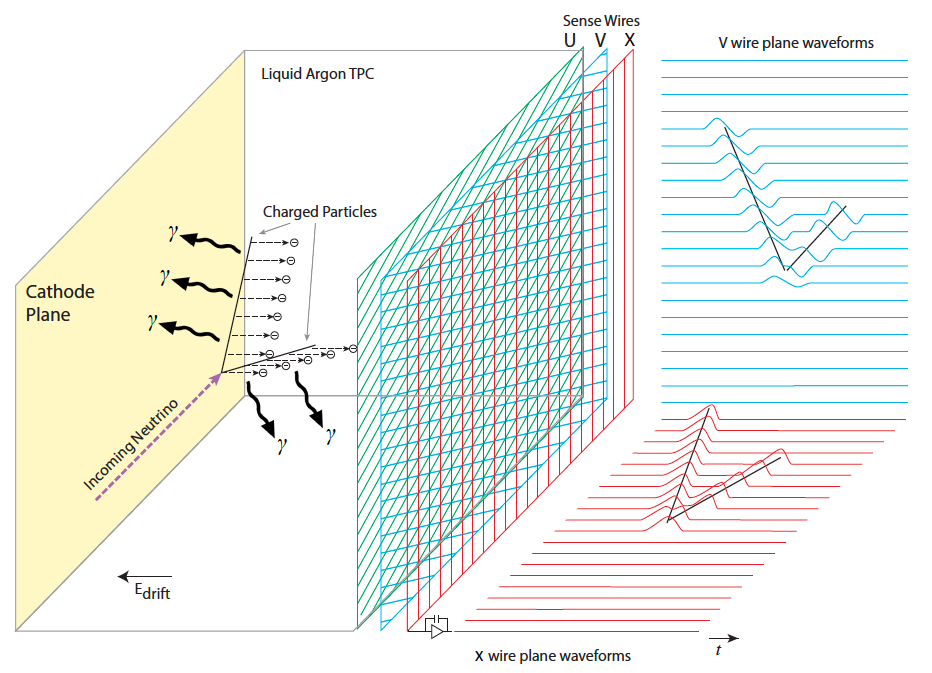
\includegraphics[width=0.75\textwidth]{graphics/TheBoPicture.png} 
\end{dunefigure}

\begin{dunefigure}[A \nominalmodsize DUNE far detector SP module.]{fig:DUNESchematic}
{Schematic of a \nominalmodsize \dword{dune} \dword{fd} \dword{spmod}, showing the alternating anode (A) and cathode (C) planes that divide the \dword{lartpc} into four separate drift volumes. The red arrows point to one top and one bottom \dword{fc} module and to the rear \dword{ewfc}.}
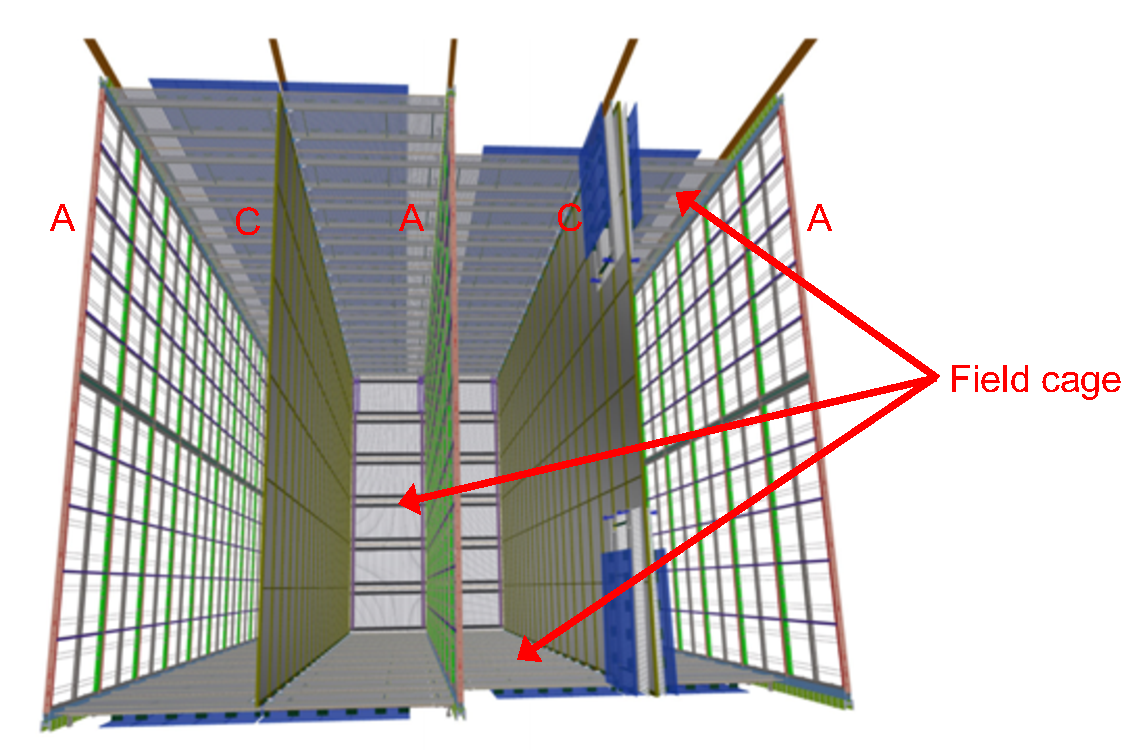
\includegraphics[width=0.65\textwidth]{DUNESchematic.pdf}
\end{dunefigure}

\Dword{pd} collector modules using \dwords{sipm} are placed in the inactive space between the innermost wire planes of the \dword{apa}s, installed through slots in a pre-wound \dword{apa} frame.  %Individual \dword{pd} modules are restricted to a profile of dimensions \SI{2.3}{cm} $\times$ \SI{11.8}{cm} $\times$ \SI{209.7}{cm}.  
There are ten \dword{pd} modules per \dword{apa} for a total of \num{1500} per \dword{spmod}.  Of these, \num{500} are mounted in central \dword{apa} frames and must collect light from both directions, % (dual-face), 
and \num{1000} are mounted in frames  near the vessel walls and collect light from only one direction. % (single-face).

\FloatBarrier
%%%%%%%%%%%%%%%%%%%%%%%%%%%%%%%%%%%%%%%%
\subsection{Dual-Phase Technology}
\label{sec:fddp-exec-splar}

The \dword{dp} operating principle, illustrated in Figure~\ref{fig:figure-label-DPprinciple} is very similar to that of the \dword{sp} design.  Charged particles that traverse the active volume of the \dword{lartpc} ionize the medium while also producing scintillation light.  The ionization electrons drift along an \efield towards a segmented anode where they deposit their charge, and where  \dwords{pd} pick up the scintillation light. 

The key differentiating concept of the \dword{dp} design is the amplification of the ionization signal in an avalanche process that takes place in a layer of argon gas above the \dword{lar}.  
In this design, shown in Figure~\ref{fig:DPdet1}, electrons drift upward toward an extraction grid just below the liquid-vapor interface. 
After reaching the grid, an \efield stronger than the \dpnominaldriftfield{} drift field extracts the electrons from the liquid up into the gas phase. Once in the gas, electrons encounter micro-pattern gas detectors, called \dwords{lem}, with high-field regions. The \dwords{lem} amplify the electrons in avalanches that occur in these high-field regions. The amplified charge is then collected and recorded on a \twod anode
consisting of two sets of %\SI{3.125}{mm}-pitch 
gold-plated copper strips that provide the $x$ and $y$ coordinates (and thus two views) of an event. 

 The extraction grid, \dword{lem}, and anode are assembled into three-layered sandwiches with precisely defined inter-stage distances and inter-alignment,  which are then connected together horizontally into \num{9}~m$^2$ modular detection units. These detection units are called \dwords{crp}.

The precision tracking and calorimetry offered by the \dword{dp} technology provides excellent capabilities for identifying interactions of interest while mitigating sources of background.  Whereas the \dword{sp} design has multiple drift volumes, the \dword{dpmod} design allows a single, fully homogeneous \dword{lar} volume with a much longer drift length.

An array of \dwords{pmt} coated with a wavelength-shifting material is located below the cathode. The \dwords{pmt} record  the time and pulse characteristics of the incident light.


\begin{dunefigure}[The DP LArTPC operating principle]{fig:figure-label-DPprinciple}{The general operating principle of the \dword{dp} \dword{lartpc}.}
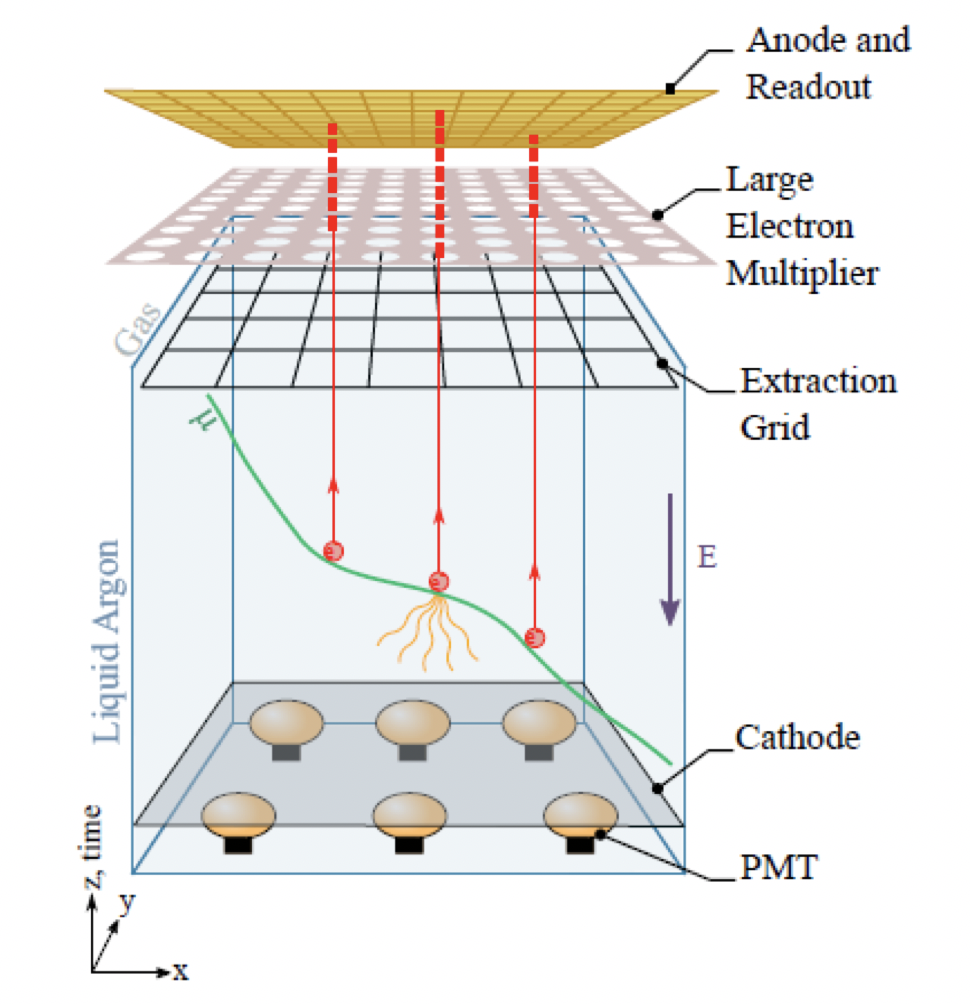
\includegraphics[width=0.5\textwidth]{dualphase-principle}
\end{dunefigure}

\begin{dunefigure}[A \nominalmodsize DUNE Far Detector DP module.]{fig:DPdet1}
  {Schematic of a \nominalmodsize DUNE \dword{fd} \dword{dp} \dword{detmodule} with cathode, \dwords{pmt}, \dword{fc}, and anode plane with \dwords{sftchimney}.}
  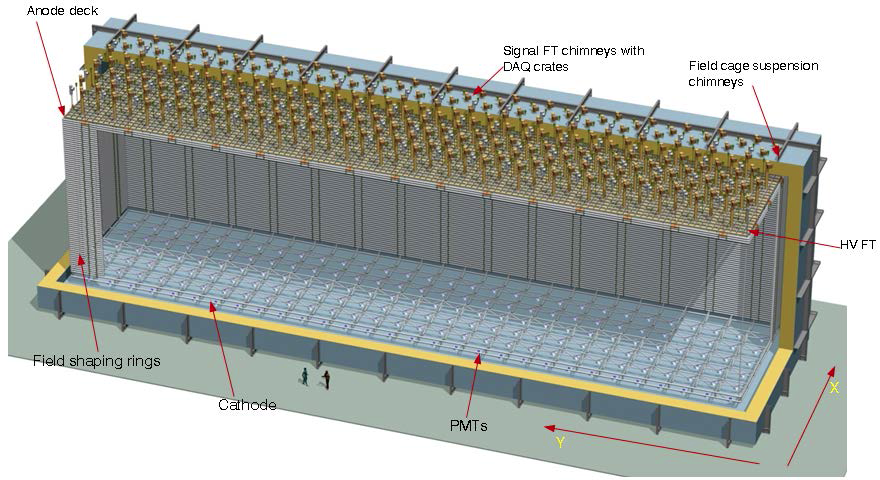
\includegraphics[width=0.9\textwidth]{DUNE-CDR-detectors-volume-optim.png}
\end{dunefigure}
\FloatBarrier
%%%%%%%%%%%%%%%%%%%%%%%


\section{The Near Detector}
\label{sec:nd-verview}

The \dword{dune} \dword{nd} will be formed from three primary detector components, listed in Table~\ref{tab:NDsumm}, and the capability for two of these components to move off the beam axis.  The three detector components -- a \dword{lartpc} called \dword{arcube} (the core component), a \dword{hpgtpc} surrounded by an \dword{ecal} (together called a \dword{mpd}), and a \dword{3dst} -- serve important individual and overlapping functions with regard to the mission of the \dword{nd}.  %Because these components have standalone features, the \dword{dune} \dword{nd} is often discussed as a suite or complex of detectors and capabilities.  
The movement off axis, called \dword{duneprism}, provides a valuable extra degree of freedom in the data and  is an integral part of the DUNE Near Detector concept.
%sometimes referred to as a fourth component. % which is discussed extensively in this report.  The power in the \dword{dune} \dword{nd} concept lies in the collective set of capabilities. % It is not unreasonable to think of the component detectors in the \dword{dune} \dword{nd} as being somewhat analogous to subsystems in a collider experiment, the difference being that, with one important exception (higher momentum muons), individual events are contained within the subsystems.  
The \dword{dune} \dword{nd} is shown schematically in the \dword{dune} \dword{nd} hall in Figure~\ref{fig:NDHallconfigs}.  Table~\ref{tab:NDsumm} provides a high-level overview of the three components of the \dword{dune} \dword{nd} along with the off-axis capability.  

\begin{dunefigure}[DUNE ND Hall with component detectors]
{fig:NDHallconfigs}
{\dword{dune} \dword{nd} Hall shown with component detectors all in the on-axis configuration (left) and with the \dword{lartpc} and \dword{mpd} in an off-axis configuration (right). The \dword{3dsts} is shown in position on the beam axis. The beam axis is shown.  The beam enters the hall at the bottom of the drawings moving from right to left.}
%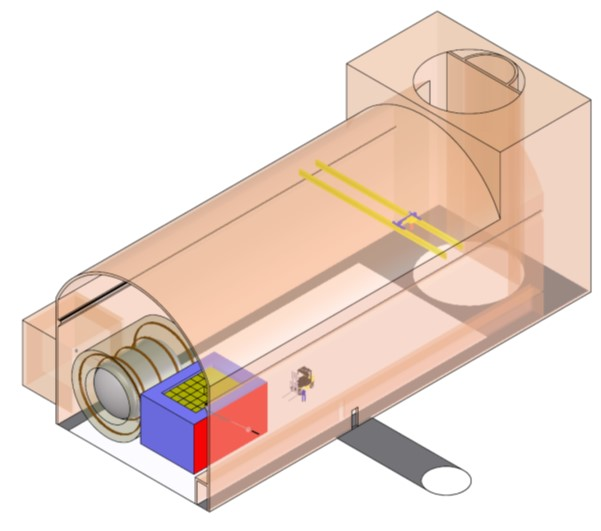
\includegraphics[width=0.49\textwidth]{graphics/NDHall_onaxis.jpg}
%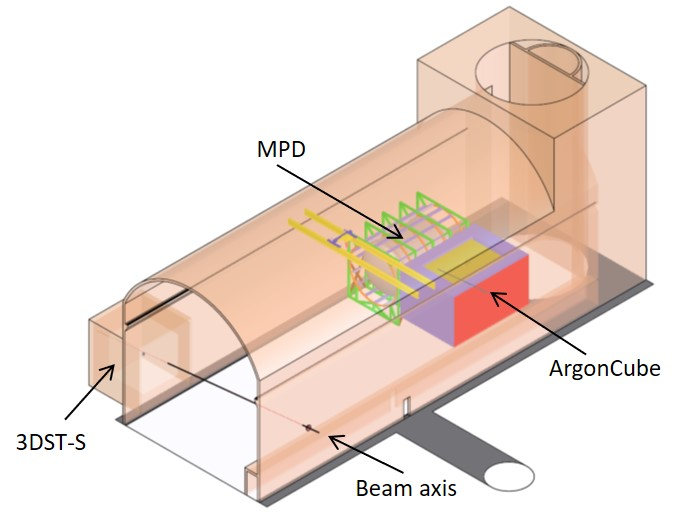
\includegraphics[width=0.49\textwidth]{graphics/NDHall_offaxis.jpg}
\end{dunefigure}

\begin{dunetable}[Components of the DUNE ND]
{p{.22\textwidth}p{.22\textwidth}p{.22\textwidth}p{.22\textwidth}}
{tab:NDsumm}{This table gives a high-level breakdown of the three major detector components and the capability of movement for the DUNE ND along with function and primary physics goals.}
Component & Essential Characteristics & Primary function & Select physics aims \\ \toprowrule
LArTPC (ArgonCube) & Mass  & Experimental control for the Far Detector & $\numu$($\overline{\nu}_{\mu}$) CC \\
          & Target nucleus Ar &  Measure unoscillated $E_\nu$ spectra   & $\nu$-e$^{-}$ scattering   \\
          &  Technology FD-like    &  Flux determination  &  $\nue +$$\overline{\nu}_{e}$ CC  \\
          &  &  &  Interaction model \\ \colhline
Multipurpose detector (MPD) & Magnetic field & Experimental control for the LArTPCs & $\numu$($\overline{\nu}_{\mu}$) CC \\
  &  Target nucleus Ar & Momentum analyze liquid Ar $\mu$ & $\nue$ CC, $\overline{\nu}_{e}$ \\
  & Low density & Measure exclusive final states with low momentum threshold & Interaction model \\  \colhline
DUNE-PRISM (capability) & LArTPC$+$MPD move off-axis & Change flux spectrum &  Deconvolve xsec*flux \\ 
 & & & Energy reponse \\
 & & & Provide FD-like energy spectrum at ND\\ 
% & & & {\   }differences \\
 & & & ID mismodeling \\ \colhline
%\dword{3dsts} 
3DST-S & On-axis & Beam flux monitor &  On-axis flux stability \\ 
  & Mass & Neutrons & Interaction model \\ 
& Magnetic field &  & A dependence \\
    & CH target & & $\nu$-e$^{-}$ scattering \\ 
\end{dunetable}



%The core part of the \dword{dune} \dword{nd} is a \dword{lartpc} called \dword{arcube}.  %The particular implementation of the \dword{lartpc} technology in this detector is described in Section~\ref{sec:exsum-nd-lartpc} below.  
The \dword{arcube} detector has the same target nucleus and shares some aspects of form and functionality with the \dword{fd}, where the differences are necessitated by the expected intensity of the beam at the \dword{nd}.  This similarity in target nucleus and, to some extent, technology, reduces sensitivity to nuclear effects and detector-driven systematic errors in the extraction of the oscillation signal at the  \dword{fd}.  The \dword{lartpc} is large enough to provide high statistics ($\num{1e8}{\numu \text{-CC events/year}}$) and a sufficient volume to provide good hadron containment.  The tracking and energy resolution, combined with the mass of the \dword{lartpc}, will allow for the measurement of the flux in the beam using several techniques, including the rare process of $\nu$-e$^{-}$ scattering.

The \dword{lartpc} begins to lose acceptance for muons above $\sim$0.7 GeV/c momentum due to lack of containment.  Because the muon momentum is a critical component of the neutrino energy determination, a magnetic spectrometer is needed downstream of the \dword{lartpc} to measure the charge sign and momentum of these muons.  In the \dword{dune} \dword{nd} concept, this function is accomplished by the multipurpose detector (\dword{mpd}) which consists of a \dword{hpgtpc} surrounded by an \dword{ecal} in a \SI{0.5}{T} magnetic field. The \dword{hpgtpc} provides a lower density medium with excellent tracking resolution for the muons from the \dword{lartpc}.  %In addition, with this choice of technology for the tracker, neutrinos interacting on the argon in the gas \dword{tpc} constitute a sample of $\nu$-Ar events that can be studied with a very low charged-particle tracking threshold and excellent resolution and systematic errors that differ from the liquid detector. The high pressure results in a sample of $\num{2e6}{\numu \text{-CC events/year}}$ for these studies. These events will be valuable for studying the charged particle activity near the interaction vertex since this detector can access lower momenta protons than the \dword{lar} detector and has better particle identification of charged $\pi$.  The lack of secondary interactions in these samples will be helpful for identifying the particles produced in the primary interaction and modeling secondary interactions in denser detectors, which are known to be important \cite{Friedland:2018vry}.
%In addition, many neutrons with high kinetic energy produced in neutrino interactions in the gaseous argon may be reconstructable via time-of-flight using the \dword{ecal}.    
%The \dword{mpd} is  discussed further in Section~\ref{ssec:exsum-nd-mpd}.


The \dword{lartpc} and \dword{mpd} can move to take data in positions off the beam axis.  This capability is referred to as \dword{duneprism}. As the detectors move off-axis, the incident neutrino flux spectrum changes, with the mean energy dropping and the spectrum becoming somewhat monochromatic.  Though the neutrino interaction rate drops off-axis, the intensity of the beam and the size of the \dword{lartpc}  combine to yield ample statistics even in the off-axis positions.
%Data taken at different off-axis angles allows for the deconvolution of the neutrino flux and interaction cross section and the mapping of the reconstructed versus true energy response of the detector.  This latter mapping is applicable at the \dword{fd} up to the level to which the near and far \dword{lar} detectors are similar.  Stated a different way, it is possible to use information from a linear combination of the different fluxes to create a data sample at the \dword{nd} with an effective neutrino energy distribution that is close to that of the oscillated spectrum at the \dword{fd}.  This data-driven technique will reduce systematic effects coming from differences in the energy spectra of the oscillated signal events in the \dword{fd} and the \dword{nd} samples used to constrain the interaction model. Finally, the off-axis degree of freedom provides a sensitivity to some forms of mismodeling in the beam and/or interaction models. %The \dword{duneprism} program is discussed further in Section~\ref{sec:exsum-nd-DP}.

The final component of the \dword{dune} \dword{nd} suite is the %\threed projection scintillator tracker spectrometer (
\dword{3dsts},  the core part of which is the \dword{3dst}.  The \dword{3dst} is a plastic scintillator detector made of \SI{1}{cm} cubes that are read out along each of three orthogonal dimensions.  %The design eliminates the typical planar-strip geometry common to detectors using scintillator, leading to improved acceptance at large angles relative to the beam direction.  The \dword{3dst} is situated along the beam axis inside an envelope of a high-resolution, normal-pressure \dwords{tpc} and an \dword{ecal}.  The entire structure is enclosed in a magnet. 
This device importantly serves as a dedicated  neutrino spectrum monitor that stays on-axis when the  \dword{lartpc} and \dword{mpd} have moved to an off-axis position. 
It also provides an excellent on-axis neutrino flux determination that can be used as an important point of comparison and a systematic crosscheck for the flux as determined by the \dword{lartpc}.
%In addition, the \dword{3dst} has very fast timing and the ability to isolate small energy depositions from neutrons in three dimensions.  This provides the capability to  incorporate neutrons in the event reconstruction using energy determination via time-of-flight with a high efficiency, expected to be useful for the low-$\nu$ flux determination. 
%The differing $A$ of the carbon target relative to argon may prove to be useful for developing models of nuclear effects and building confidence in the interaction model and the size of numerous systematic errors.  Recent electron scattering results on C, Ti, and Ar targets are described very well by the SuSAv2-MEC superscaling framework and this is expected to be applicable to neutrinos~\cite{Barbaro:2019vsr}. 

\subsection{Near Detector}



The near detector will be located \SI{575}{m} from the target. It will consist of a \lartpc followed by a fine-grained magnetic spectrometer. The \lartpc will use pixel readout to deal with the high occupancy from neutrino events in the intense LBNF beam. The details of the magnetic spectrometer will use a high pressure argon gas TPC.
The goal for the near detector group is to produce a \dword{cdr} around the end of 2019, and a \dword{tdr} in 2020, consistent with the planned construction schedule for the ND. The ND summary included in this volume shows that the planned ND should allow us to reach the goals of the primary neutrino oscillation program of DUNE.



The collaboration is in now in the final stages of constructing two large prototype detectors (called \dwords{protodune}), one employing \single readout (\dword{pdsp}) and the other employing \dual readout (\dword{pddp}). Each is approximately one-twentieth of a DUNE \dword{detmodule}, but uses components identical in size to those of the full-scale module. \dword{pdsp} has the same \spmaxdrift maximum drift length as the full \dword{spmod}. \dword{pddp} has a \SI{6}{m} maximum drift length, half of that planned for the \dword{dpmod}. 

These large-scale prototypes will allow us to validate key aspects of the TPC designs, test engineering procedures, and collect valuable calibration data using a hadron test beam. The following list includes the key goals of the \dword{protodune} program:
\begin{enumerate}
\item Test production of components:
\begin{itemize}
\item stress testing of the production and quality
assurance processes of detector components,
\item mitigation of the associated risks for the far detector.
\end{itemize}
\item Validate installation procedures:
\begin{itemize}
\item test of the interfaces between the detector elements,
\item mitigation of the associated risks for the far detector.
\end{itemize}
\item Detector operation with cosmic rays:
\begin{itemize}
\item validation of the detector designs and
performance.
\end{itemize}
\item Collection of test beam data:
\begin{itemize}
\item measurements of essential physics response of the detector.
\end{itemize}
\end{enumerate}

Items \numrange{1}{3} are required as input to the \dword{tdr}. Item 4, collection and the corresponding analysis of test beam data, will be vital to DUNE's physics program, but is not required for the TDR.

The full DUNE far detector requires four modules. For the \dword{tdr}, we will describe plans for at least the first two of these modules. Based on our current expectations, we hope to present a plan for two \dwords{spmod}, one of which will be the first module installed, and one \dword{dpmod}. At the time of the \dword{tdr}, it is likely that resources for the fourth \dword{detmodule} will remain to be identified. 


%Sample figure to copy and edit, %Figure~\ref{fig:map}:



Sample table to copy and edit, Table~\ref{tab:execosctable}:

\begin{dunetable}[Required exposures to reach oscillation physics
  milestones]{lcc}{tab:execosctable}{The exposure in mass (kt) $\times$ proton beam power
    (MW) $\times$ time (years) and calendar years assuming the staging plan described in this chapter needed to reach certain oscillation physics
    milestones. The numbers are for normal hierarchy using the NuFit 2016 best fit values of the known oscillation parameters.  }
Physics milestone & Exposure  & Exposure \\ \rowtitlestyle
  & (\ktMWyr{}) & (years)  \\ \toprowrule 
  $1^\circ$ $\theta_{23}$ resolution ($\theta_{23} = 42^\circ$) & 29  &  1\\ \colhline
  CPV at $3\sigma$ ($\delta_{\rm CP} = -\pi/2$)  & 77 &  3\\ \colhline
  \dword{mh} at  $5\sigma$ (worst point) & 209 & 6 \\ \colhline
  $10^\circ$ $\delta_{\rm CP}$ resolution ($\delta_{\rm CP} = 0$) & 252 & %5 
  6.5 \\ \colhline
  ($\sin^2 2 \theta_{13} = 0.084 \pm 0.003$) &  &  \\  
\end{dunetable}
